\chapter{Schedule Properties and Argumentation}
\label{properties}

Schedule properties such as feasibility are modelled using frameworks to explain the satisfaction of properties. The definitions of efficiency and fixed decision frameworks extend from the definition of the feasibility framework. In this chapter, this extension is interesting because, this can be generalised to reason about arbitrary number of properties, using a extended framework. We apply this generalisation to interval scheduling to illustrate applications of argumentation.
\linespace 
We use stability over other notions of good extensions such as admissibility and completeness to accurately model schedule constraints. This is because we know that existing problems, such as the stable marriage problem can be modelling using stability \cite{aa}.

\section{Frameworks}
\label{unionframeworks}

In order to reason about an arbitrary number of properties, we inductively construct the expressible properties over an extendable framework, denoted by $\pair{Args}{\rightsquigarrow_0}$. An arbitrary property $P_k$ is modelled by the framework $\pair{Args}{\rightsquigarrow_k}$. To be correct, we must preserve that extension $E$ is stable on $\pair{Args}{\rightsquigarrow_0\cup\rightsquigarrow_k}$ if $E$ is also stable on $\pair{Args}{\rightsquigarrow_0}$ and $P(S)$ holds. Let $\rightsquigarrow,\rightsquigarrow_1,\rightsquigarrow_2\subseteq Args^2$ be arbitrary frameworks.

\begin{definition}
	A framework $\pair{Args}{\rightsquigarrow}$ stability-models a schedule property $P$ iff for all extensions $E$ and corresponding schedules $S$, $E$ is stable on $\pair{Args}{\rightsquigarrow}$ $\Leftrightarrow$ $P(S)$
\end{definition}

\begin{definition}
	A framework $\pair{Args}{\rightsquigarrow}$ conflict-models a schedule property $P$ iff for all extensions $E$ and corresponding schedules $S$, $E$ is conflict-free on $\pair{Args}{\rightsquigarrow}$ $\Leftrightarrow$ $P(S)$
\end{definition}

These definitions are used to make concise proofs.

\begin{proposition}
	$\rightsquigarrow_F$ stability-models feasibility \cite{aes}.
\end{proposition}

\begin{proposition}
	$\rightsquigarrow_S$ stability-models feasibility and efficiency \cite{aes}.
\end{proposition}

\begin{proposition}
	$\rightsquigarrow_D$ stability-models feasibility and satisfaction of fixed decisions \cite{aes}.
\end{proposition}

\begin{definition}
	\label{conflictmodellable}
	
	A schedule property $P$ is conflict-modellable iff there exists a framework that conflict-models $P$.
\end{definition}

\begin{definition}
	\label{stablemodellable}
	
	A schedule property $P$ is stability-modellable iff there exists a framework that stability-models $P$.
\end{definition}

Definitions \ref{conflictmodellable} and \ref{stablemodellable} intuitively specifies that a property can be verified using AAFs. In context of schedules, stability-modellable constraints are useful because it shows an application of argumentation. However, a stability-modellable constraint is not equivalent to using any argumentation framework. For example, the constraint $a+b+c+d\leq 2$ is not stability-modellable because stability does not count the number of conflicting attacks or unattacked arguments. But in value-based argumentation frameworks, it is possible to define an altered form of stability that is sensitive to attack weights. To find an extension in this weighted-stability, this problem can be reduced into a subset sum problem, which cannot be solved in polynomial time.

\begin{lemma}
	\label{buildconflictfreeness}
	$E$ is conflict-free on $\pair{Args}{\rightsquigarrow_1}$ and on $\pair{Args}{\rightsquigarrow_2}$ iff $E$ is conflict-free on $\pair{Args}{\rightsquigarrow_1\cup\rightsquigarrow_2}$.	

	\begin{proof}
		To prove the forward implication, assume $E$ is conflict-free on $\pair{Args}{\rightsquigarrow_1}$ and on $\pair{Args}{\rightsquigarrow_2}$. To aim for a contradiction, assume $E$ is not conflict-free on $\pair{Args}{\rightsquigarrow_1\cup\rightsquigarrow_2}$. Then there exists $e_1,e_2\in E$ such that $e_1(\rightsquigarrow_1\cup\rightsquigarrow_2)e_2$. Then $e_1\rightsquigarrow_1 e_2$ or $e_1\rightsquigarrow_2 e_2$. Both cases lead to a contradiction, so $E$ is conflict-free on $\pair{Args}{\rightsquigarrow_1\cup\rightsquigarrow_2}$.
		\linespace
		To prove the backward implication, assume $E$ is conflict-free on $\pair{Args}{\rightsquigarrow_1\cup\rightsquigarrow_2}$. To aim for a contradiction, assume $E$ is not conflict-free on $\pair{Args}{\rightsquigarrow_1}$. Then there exists $e_1,e_2\in E$ such that $e_1\rightsquigarrow_1 e_2$. Then $e_1(\rightsquigarrow_1\cup\rightsquigarrow_2)e_2$, which contradicts the most recent assumption. Therefore, $E$ is conflict-free on $\pair{Args}{\rightsquigarrow_1}$, and also conflict-free on $\pair{Args}{\rightsquigarrow_2}$ by similar argument.
	\end{proof}
\end{lemma}

\begin{figure}[H]
	\begin{center}
		\begin{tikzpicture}
			\node[node](a) at (0, 2){a};
			\node[node, shaded](b) at (2, 2){b};
			\node[node](c) at (2, 0){c};
			\node[node, shaded](d) at (0, 0){d};
			\draw[arrow](a) -- (c);
			\draw[arrow](c) -- (b);
			\draw[arrow](d) -- (a);
		\end{tikzpicture}\hspace{1cm}
		\begin{tikzpicture}
			\node[node](a) at (0, 2){a};
			\node[node, shaded](b) at (2, 2){b};
			\node[node](c) at (2, 0){c};
			\node[node, shaded](d) at (0, 0){d};
			\draw[arrow, dashed](b) -- (a);
			\draw[arrow, dashed](c) -- (b);
			\draw[arrow, dashed](c) -- (d);
		\end{tikzpicture}\hspace{1cm}
		\begin{tikzpicture}
			\node[node](a) at (0, 2){a};
			\node[node, shaded](b) at (2, 2){b};
			\node[node](c) at (2, 0){c};
			\node[node, shaded](d) at (0, 0){d};
			\draw[arrow](a) -- (c);
			\draw[arrow](c) -- (b);
			\draw[arrow](d) -- (a);
			\draw[arrow, dashed](b) -- (a);
			\draw[arrow, dashed](c) -- (b);
			\draw[arrow, dashed](c) -- (d);
		\end{tikzpicture}
	\end{center}
	\caption{Lemma \ref{buildconflictfreeness} states that given a conflict-free extension over two attack sets on the same arguments, the extension is conflict-free on the merged framework. The figure illustrates this by merging the left and middle frameworks to produce the right framework.}
\end{figure}

\begin{lemma}
	\label{buildstability}
	If $E$ is stable on $\pair{Args}{\rightsquigarrow_1}$ and $E$ is conflict-free on $\pair{Args}{\rightsquigarrow_2}$, then $E$ is stable on $\pair{Args}{\rightsquigarrow_1\cup\rightsquigarrow_2}$.
	
	\begin{proof}
		Assume $E$ is stable on $\rightsquigarrow_1$ and $E$ is conflict-free on $\rightsquigarrow_2$. By definition of stability, $\forall a\in Args\setminus E\ \exists e\in E\ e\rightsquigarrow_1 a$. Then $\forall a\in Args\setminus E\ \exists e\in E\ e(\rightsquigarrow_1\cup\rightsquigarrow_2)a$. So every argument not in $E$ is attacked by some argument in $E$. $E$ is conflict-free on $\rightsquigarrow_1$ because $E$ is stable on $\rightsquigarrow_1$. Since $E$ is conflict-free on $\rightsquigarrow_1$ and on $\rightsquigarrow_2$, we use Lemma \ref{buildconflictfreeness} to show that $E$ is also conflict-free on $(\rightsquigarrow_1\cup\rightsquigarrow_2)$. Therefore $E$ is stable on $\pair{Args}{\rightsquigarrow_1\cup\rightsquigarrow_2}$.
	\end{proof}
\end{lemma}

\begin{figure}[H]
	\begin{center}
		\begin{tikzpicture}
		\node[node](a) at (0, 2){a};
		\node[node](b) at (2, 2){b};
		\node[node, shaded](c) at (2, 0){c};
		\node[node, shaded](d) at (0, 0){d};
		\draw[arrow](a) -- (c);
		\draw[arrow](c) -- (b);
		\draw[arrow](d) -- (a);
		\end{tikzpicture}\hspace{1cm}
		\begin{tikzpicture}
		\node[node](a) at (0, 2){a};
		\node[node](b) at (2, 2){b};
		\node[node, shaded](c) at (2, 0){c};
		\node[node, shaded](d) at (0, 0){d};
		\draw[arrow, dashed](b) -- (a);
		\draw[arrow, dashed](b) -- (d);
		\end{tikzpicture}\hspace{1cm}
		\begin{tikzpicture}
		\node[node](a) at (0, 2){a};
		\node[node](b) at (2, 2){b};
		\node[node, shaded](c) at (2, 0){c};
		\node[node, shaded](d) at (0, 0){d};
		\draw[arrow](a) -- (c);
		\draw[arrow](c) -- (b);
		\draw[arrow](d) -- (a);
		\draw[arrow, dashed](b) -- (a);
		\draw[arrow, dashed](b) -- (d);
		\end{tikzpicture}
	\end{center}
	\caption{Lemma \ref{buildstability} allows stable extensions of attacks to grow with conflict-free attacks. The left framework is the base framework and the right framework is the extended framework.}
\end{figure}

\begin{lemma}
	\label{reduceconflictfreeness}
	If $E$ is stable on $\pair{Args}{\rightsquigarrow_1\cup\rightsquigarrow_2}$, then $E$ is conflict-free on $\pair{Args}{\rightsquigarrow_1}$.
	
	\begin{proof}
		Assume $E$ is stable on $\pair{Args}{\rightsquigarrow_1\cup\rightsquigarrow_2}$. By definition of stability, $E$ is conflict-free on $\pair{Args}{\rightsquigarrow_1\cup\rightsquigarrow_2}$.  By Lemma \ref{buildconflictfreeness}, $E$ is conflict-free on $\pair{Args}{\rightsquigarrow_1}$.
	\end{proof}
\end{lemma}

\begin{figure}[H]
	\begin{center}
		\begin{tikzpicture}
			\node[node](a) at (0, 2){a};
			\node[node](b) at (2, 2){b};
			\node[node, shaded](c) at (2, 0){c};
			\node[node, shaded](d) at (0, 0){d};
			\draw[arrow](a) -- (c);
			\draw[arrow](b) -- (a);
			\draw[arrow](c) -- (b);
			\draw[arrow](d) -- (a);
		\end{tikzpicture}\hspace{3cm}
		\begin{tikzpicture}
			\node[node](a) at (0, 2){a};
			\node[node](b) at (2, 2){b};
			\node[node, shaded](c) at (2, 0){c};
			\node[node, shaded](d) at (0, 0){d};
			\draw[arrow](a) -- (c);
			\draw[arrow](c) -- (b);
		\end{tikzpicture}
	\end{center}
	\caption{Lemma \ref{reduceconflictfreeness} states that given a stable extension, removing attacks preserves the extension's conflict-freeness, as shown from left to right.}
\end{figure}

\begin{lemma}
	\label{reducestability}
	If $E$ is stable on $\pair{Args}{\rightsquigarrow_1\cup\rightsquigarrow_2}$ and $\forall a\in Args\setminus E\ (\exists e\in E\ e\rightsquigarrow_2 a)\implies(\exists e\in E\ e\rightsquigarrow_1 a)$, then $E$ is stable on $\pair{Args}{\rightsquigarrow_1}$.
	
	\begin{proof}
		\begin{flalign*}
			&E\text{ is stable on }\pair{Args}{\rightsquigarrow_1\cup\rightsquigarrow_2}&\\
			&\land\forall a\in Args\setminus E\ (\exists e\in E\ e\rightsquigarrow_2 a)\implies(\exists e\in E\ e\rightsquigarrow_1 a)\\
			\implies&E\text{ is conflict-free on }\pair{Args}{\rightsquigarrow_1\cup\rightsquigarrow_2}\\
			&\land\forall a\in Args\setminus E\ \exists e\in E\ e(\rightsquigarrow_1\cup\rightsquigarrow_2)\\
			&\land\forall a\in Args\setminus E\ (\exists e\in E\ e\rightsquigarrow_2 a)\implies(\exists e\in E\ e\rightsquigarrow_1 a)\\
			&\textit{definition of stability}\\
			\implies&E\text{ is conflict-free on }\pair{Args}{\rightsquigarrow_1}\\
			&\land\forall a\in Args\setminus E\ \exists e\in E\ (e\rightsquigarrow_1 a\lor e\rightsquigarrow_2 a)\\
			&\land\forall a\in Args\setminus E\ (\exists e\in E\ e\rightsquigarrow_2 a)\implies(\exists e\in E\ e\rightsquigarrow_1 a)\\
			&\textit{definition of $\cup$}\\
			\implies&E\text{ is conflict-free on }\pair{Args}{\rightsquigarrow_1}\\
			&\land\forall a\in Args\setminus E\ ((\exists e\in E\ e\rightsquigarrow_1 a)\lor(\exists e\in E\ e\rightsquigarrow_2 a))\\
			&\land\forall a\in Args\setminus E\ (\exists e\in E\ e\rightsquigarrow_2 a)\implies(\exists e\in E\ e\rightsquigarrow_1 a)\\
			&\textit{distribute $\lor$ over $\exists$}\\
			\implies&E\text{ is conflict-free on }\pair{Args}{\rightsquigarrow_1}\\
			&\land\forall a\in Args\setminus E\ ((\exists e\in E\ e\rightsquigarrow_1 a)\lor(\exists e\in E\ e\rightsquigarrow_1 a))\\
			&\textit{substitute $\rightsquigarrow_2$ to $\rightsquigarrow_1$}\\
			\implies&E\text{ is conflict-free on }\pair{Args}{\rightsquigarrow_1}\\
			&\textit{idempotency of $\lor$}\\
			&\land\forall a\in Args\setminus E\ \exists e\in E\ e\rightsquigarrow_1 a\\
			\implies&E\text{ is stable on }\pair{Args}{\rightsquigarrow_1}\\
			&\textit{definition of stability}
		\end{flalign*}
	\end{proof}
\end{lemma}

\begin{figure}[H]
	\begin{center}
		\begin{tikzpicture}
		\node[node](a) at (0, 2){a};
		\node[node](b) at (2, 2){b};
		\node[node, shaded](c) at (2, 0){c};
		\node[node, shaded](d) at (0, 0){d};
		\draw[arrow, dashed](c) -- (a);
		\draw[arrow](c) -- (b);
		\draw[arrow](d) -- (a);
		\draw[arrow, dashed](d) -- (b);
		\end{tikzpicture}\hspace{3cm}
		\begin{tikzpicture}
		\node[node](a) at (0, 2){a};
		\node[node](b) at (2, 2){b};
		\node[node, shaded](c) at (2, 0){c};
		\node[node, shaded](d) at (0, 0){d};
		\draw[arrow](c) -- (b);
		\draw[arrow](d) -- (a);
		\end{tikzpicture}
	\end{center}
	\caption{Lemma \ref{reducestability} states that given a stable extension, removing attacks on multi-attacked arguments preserves the extension's stability, as shown from left to right.}
\end{figure}

\begin{theorem}[\textbf{Union of modelling frameworks}]
	\label{modelling}
	Let $P_0,...,P_K$ be schedule properties with $K$ properties. Let $P_{\intset{i,j}}$ be an aggregate schedule property where for all schedules $S$, $P_{\intset{i, j}}(S)\iff\forall k\in\intset{i,j}\ P_k(S)$.
	\linespace
	If $\rightsquigarrow_0$ stability-models $P_0$, and $\forall k\in\intset{1,K}\ \rightsquigarrow_k$ conflict-models $P_k$, and for all extensions $E$, $\forall a\in Args\setminus E\ \forall k\in\intset{1,K}\ \big((\exists e\in E\ e\rightsquigarrow_k a)\implies(\exists e\in E\ e\rightsquigarrow_0 a)\big)$, then $\left(\bigcup_{k=0}^K\rightsquigarrow_k\right)$ stability-models $P_{\intset{0,K}}$.
	
	\begin{proof}
		Take arbitrary $K\in\mathbb{N}$. To prove forward implication:
		\begin{enumerate}
			\item$\rightsquigarrow_0$ stability-models $P_0$\hfill given
			\item$\forall k\in\intset{1,K}\ \rightsquigarrow_k$ conflict-models $P_k$\hfill given
			\item$\forall a\in Args\setminus E\ \forall k\in\intset{1,K}\ \big((\exists e\in E\ e\rightsquigarrow_k a)\implies(\exists e\in E\ e\rightsquigarrow_0 a)\big)$\\\null\hfill given
			\item$E$ is stable on $\pair{Args}{\bigcup_{k=0}^K\rightsquigarrow_k}$\hfill assumption
			\item$\forall a\in Args\setminus E\ \left(\left(\exists e\in E\ e\left(\bigcup_{k=0}^K\rightsquigarrow_k\right) a\right)\implies(\exists e\in E\ e\rightsquigarrow_0 a)\right)$\\\null\hfill 3
			\item$E$ is stable on $\pair{Args}{\rightsquigarrow_0}$\hfill lemma \ref{reducestability}, 4, 5
			\item$P_0(S)$\hfill 1, 6
			\item Take arbitrary $k\in\intset{1,K}$
			\begin{level}
				\item$E$ is conflict-free on $\pair{Args}{\rightsquigarrow_k}$\hfill lemma \ref{reduceconflictfreeness}, 4
				\item$P_k$(S)\hfill 2, 9
			\end{level}
			\item$\forall k\in\intset{1,K}\ P_k(S)$\hfill 8, 10
			\item$P_{\intset{0,K}}(S)$ \hfill 7, 11
		\end{enumerate}
	
		To prove backward implication:
		\begin{enumerate}
			\item$\rightsquigarrow_0$ stability-models $P_0$\hfill given
			\item$\forall k\in\intset{1,K}\ \rightsquigarrow_k$ conflict-models $P_k$\hfill given
			\item$P_{\intset{0,K}}(S)$\hfill assumption
			\item$P_0(S)$\hfill 3
			\item$E$ is stable on $\pair{Args}{\rightsquigarrow_0}$\hfill 1, 4
			\item Recursively over $k\in\intset{1,K}$
			\begin{level}
				\item $P_k(S)$\hfill 3
				\item $E$ is conflict-free on $\pair{Arg}{\rightsquigarrow_k}$\hfill 2, 7
				\item $E$ is stable on $\pair{Arg}{\bigcup_{k'=0}^k\rightsquigarrow_{k'}}$\hfill lemma \ref{buildstability}, 5, 8
			\end{level}
			\item $E$ is stable on $\pair{Arg}{\bigcup_{k=0}^K\rightsquigarrow_k}$\hfill 6, 9
		\end{enumerate}
	\end{proof}
\end{theorem}

\begin{figure}[H]
	\begin{center}
		\begin{tikzpicture}
			\node[node, shaded](a) at (0, 1.5){a};
			\node[node](b) at (1.5, 1.5){b};
			\node[node, shaded](c) at (1.5, 0){c};
			\node[node](d) at (0, 0){d};
			\draw[arrow](a) -- (b);
			\draw[arrow](b) -- (a);
			\draw[arrow](c) -- (d);
			\draw[arrow](d) -- (c);
			\draw(-0.5,-0.5) rectangle (2,2);
			\node at (0.8, -0.8){stability-models $P_0$};
		\end{tikzpicture}\raisebox{1.4cm}{\huge{$\land$}}
		\begin{tikzpicture}
			\node[node, shaded](a) at (0, 1.5){a};
			\node[node](b) at (1.5, 1.5){b};
			\node[node, shaded](c) at (1.5, 0){c};
			\node[node](d) at (0, 0){d};
			\draw[arrow](b) -- (c);
			\draw(-0.5,-0.5) rectangle (2,2);
			\node at (0.8, -0.8){conflict-models $P_1$};
		\end{tikzpicture}\raisebox{1.4cm}{\huge{$\land$ ... $\land$}}
		\begin{tikzpicture}
			\node[node, shaded](a) at (0, 1.5){a};
			\node[node](b) at (1.5, 1.5){b};
			\node[node, shaded](c) at (1.5, 0){c};
			\node[node](d) at (0, 0){d};
			\draw[arrow](b) -- (d);
			\draw(-0.5,-0.5) rectangle (2,2);
			\node at (0.8, -0.8){conflict-models $P_K$};
		\end{tikzpicture}\linespace
		{\huge{$\Updownarrow$}}
		\linespace
		\begin{tikzpicture}
			\node[node, shaded](a) at (0, 2){a};
			\node[node](b) at (2, 2){b};
			\node[node, shaded](c) at (2, 0){c};
			\node[node](d) at (0, 0){d};
			\draw[arrow](a) -- (b);
			\draw[arrow](b) -- (a);
			\draw[arrow](b) -- (c);
			\draw[arrow](b) -- (d);
			\draw[arrow](c) -- (d);
			\draw[arrow](d) -- (c);
			\draw(-0.5,-0.5) rectangle (2.5, 2.5);
			\node at (1, -0.8){stability-models $P_{\intset{0,K}}$};
		\end{tikzpicture}
		\vspace{-\baselineskip}
	\end{center}
	\caption{Theorem \ref{modelling} allows manipulation of an aggregate property, $P_{\intset{0,K}}$ from carefully extending frameworks, while preserving stability. This theorem is a key statement in framing argumentation semantics for arbitrary scheduling problems.}
\end{figure}

Theorem \ref{modelling} cannot be applied to $\rightsquigarrow_S$ or $\rightsquigarrow_D$ because they remove attacks from the $\rightsquigarrow_F$. The theorem does not capture removal of attacks from a commonly-extendable framework because there is ambiguity between the order of removal and insertion of attacks. Formally, $(\rightsquigarrow\cup \rightsquigarrow^+)\setminus \rightsquigarrow^-\neq (\rightsquigarrow\setminus\rightsquigarrow^-)\cup\rightsquigarrow^+$ for arbitrary frameworks $\rightsquigarrow,\rightsquigarrow^-,\rightsquigarrow^+$.

\section{Interval Scheduling}
\label{interval}

Makespan schedules are extended to discrete time-indexed interval scheduling. We will show an application of Theorem \ref{modelling} to interval scheduling. Let $T$ be the exclusive upper-bound of indexed time where $\mathcal{T}=\{0,...,T-1\}$. The assignment matrix $\mathbf{x}\in\mathcal{M}\times\mathcal{J}\times\mathcal{T}$ is extended such that $x_{i,j,t}=1$ iff job $j$ is starts work on machine $i$ at time $t$. Each machine job pair $\pair{i}{j}$ has a start time $s_{i,j}\in\mathcal{T}^{mn}$ and finish time $f_{i,j}\in\{0,...,T\}^{mn}$, where $j$ must be completed within the $[s_{i,j},f_{i,j})$ interval. The objective is to minimise the total completion time.

\begin{align*}
	\min_{\mathbf{x}}\ &C_{\max}\text{ subject to:}\\
	\forall i\in\mathcal{M}\ \forall j\in\mathcal{J}\ \forall t\in\mathcal{T}\ &C_{\max}\geq x_{i,j,t}(t+p_j)\\
	\forall j\in\mathcal{J}\ &\sum_{i\in\mathcal{M}}\sum_{t\in\mathcal{T}}x_{i,j,t}=1&\alpha\\
	\forall i\in\mathcal{M}\ \forall t\in\mathcal{T}\ &\sum_{j\in\mathcal{J}}\sum_{t'=\max\{t-p_j+1,0\}}^t x_{i,j,t'}\leq 1&\beta\\
	\forall i\in\mathcal{M}\ \forall j\in\mathcal{J}\ \forall t\in\{0,...,s_{i,j}-1\}\ &x_{i,j,t}=0&\gamma\\
	\forall i\in\mathcal{M}\ \forall j\in\mathcal{J}\ \forall t\in\{f_{i,j}-p_j+1,...,T-1\}\ &x_{i,j,t}=0&\delta\\
	\forall\triple{i}{j}{t}\in D^-\ &x_{i,j,t}=0&\varepsilon\\
	\forall\triple{i'}{j}{t'}\in D^+\ \forall i\in\mathcal{M}\setminus\{i'\}\ \forall t\in\mathcal{T}\ &x_{i,j,t}=0&\zeta\\
	\forall\triple{i}{j}{t'}\in D^+\ \forall t\in\mathcal{T}\ &&\\
	t\leq t'-p_j\lor t\geq t'+p_j\implies&x_{i,j,t}=0&\eta\\
\end{align*}

$\alpha$ models feasibility, that all jobs must be allocated. $\beta$ models that machines cannot process multiple jobs at the same time. $\gamma$ and $\delta$ models the restriction of start and end times respectively. $\varepsilon$ and $\zeta$ models negative and positive fixed decisions respectively. Equivalently, $\zeta$ can be modelled by $\forall\triple{i}{j}{t'}\in D^+\ \exists t\in\mathcal{T}\ x_{i,j,t}=1$. $\zeta$ is defined as such to simplify the proof that the union of these properties is modellable. $\eta$ models enforces that $j$ is working on $i$ at $t$, but does not specify the when $j$ starts. Note that $\gamma,\delta,\zeta$ and $\eta$ can be modelled using $\varepsilon$. We use more constants to give better explanations, because each constraint have different explanations. For argumentation, let $Args=\mathcal{M}\times\mathcal{J}\times\mathcal{T}$.

\begin{figure}[H]
	\begin{center}
		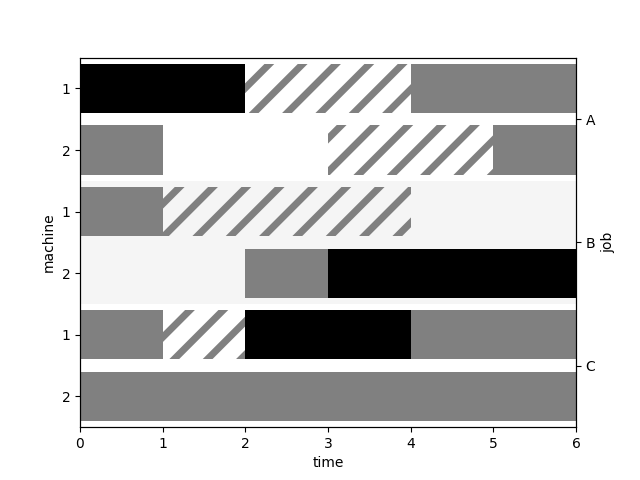
\includegraphics[width=.8\linewidth]{figures/interval.png}	
	\end{center}
	\caption{An interval schedule, where black areas are assignments and the grey areas show invalid slots because of negative fixed decisions or other job assignees.}
\end{figure}

\begin{definition}
	\label{intervalalpha}
	
	Let $\rightsquigarrow_\alpha$ be the base-feasibility framework such that $\triple{i}{j}{t}\rightsquigarrow_\alpha\triple{i'}{j'}{t'}\Leftrightarrow i\neq i'\land j=j'\land t\neq t'$ 
\end{definition}

$\rightsquigarrow_\alpha$ can be interpreted as an generalisation of $\rightsquigarrow_F$ with time.

\begin{lemma}
	\label{stabilityalpha}
	$\rightsquigarrow_\alpha$ stability-models $\alpha$.
	
	\begin{proof}
		To prove forward implication: $E$ is stable on $\pair{Args}{\rightsquigarrow_\alpha}$. Take arbitrary $j\in\mathcal{J}$. To aim to contradict, assume $\sum_{i\in\mathcal{M}}\sum_{t\in\mathcal{T}}x_{i,j,t}>1$. Then $\exists\triple{i}{j}{t},\triple{i'}{j}{t'}\in E$ where $x_{i,j,t}=1$ and $x_{i',j,t'}=1$ such that $i\neq i'$ or $t\neq t'$. By definition of $\rightsquigarrow_\alpha$, $\triple{i}{j}{t}\rightsquigarrow_\alpha\triple{i'}{j}{t'}$. Hence $E$ is not conflict-free, then $E$ is not stable. By contradiction, $\sum_{i\in\mathcal{M}}\sum_{t\in\mathcal{T}}x_{i,j,t}\leq 1$. To aim to contradict, assume $\sum_{i\in\mathcal{M}}\sum_{t\in\mathcal{T}}x_{i,j,t}=0$. Then $\forall i\in\mathcal{M}\ \forall t\in\mathcal{T}\ x_{i,j,t}=0$. Then $\forall i\in\mathcal{M}\ \forall t\in\mathcal{T}\ \triple{i}{j}{t}\not\in E$. Then $E$ is not stable. By contradiction, $\sum_{i\in\mathcal{M}}\sum_{t\in\mathcal{T}}x_{i,j,t}>0$. Therefore $\alpha$ holds.
		\linespace
		To prove backward implication: From $\alpha$, there is exactly one $i\in\mathcal{M}$ and $t\in\mathcal{T}$ such that $x_{i,j,t}=1$. So $E$ is conflict free. Also, for all $j$, $\triple{i}{j}{t}\in E$ attacks every other $\pair{i}{t}$, so $E$ is stable.
	\end{proof}
\end{lemma}

\begin{definition}
	\label{intervalbeta}
	
	Let $\rightsquigarrow_\beta$ be the sequential-feasibility framework such that $\triple{i}{j}{t}\rightsquigarrow_\beta\triple{i'}{j'}{t'}\Leftrightarrow i=i'\land(t'\leq t\leq t'+p_j'\lor t\leq t'<t+p_j)$.
\end{definition}

\begin{lemma}
	\label{conflictfreenessbeta}
	$\rightsquigarrow_\beta$ conflict-models $\beta$.
	
	\begin{proof}
		To show $E$ is conflict-free implies $\beta$: Take arbitrary $i\in\mathcal{M}$, $t\in\mathcal{T}$. To aim for a contradiction, assume $\sum_{j\in\mathcal{J}}\sum_{t'\in\max\{t-p_j+1,0\}}x_{i,j,t'}\geq 2$. Then there exists some $j_1,j_2\in\mathcal{J}$ and some $t_1,t_2\in\mathcal{T}$ such that $0\leq t_1,t_2\leq t$ and $x_{i,j_1,t_1}+x_{i,j_2,t_2}=2$. Then $\triple{i}{j_1}{t_1}\in E$ and $\triple{i}{j_2}{t_2}\in E$. By conduction of $\beta$, then either $t_1\leq t_2\leq t_1+p_1$ or $t_2\leq t_1\leq t_2+p_2$. By definition of $\rightsquigarrow_\beta$, $\triple{i}{j_1}{t_1}\rightsquigarrow_\beta\triple{i}{j_2}{t_2}$. But this contradicts that $E$ is conflict-free. Therefore $\beta$ holds.
		\linespace
		To show $\beta$ implies $E$ is conflict-free: Assume $\beta$ holds. Take arbitrary $i\in\mathcal{M}$, $t\in\mathcal{T}$. Then there does not exists overlapping jobs $j_1$ and $j_2$ such that $x_{i,j_1,t_1}+x_{i,j_2,t_2}=2$. Then $\triple{i}{j_1}{t_1}\not\in E$ and $\triple{i}{j_2}{t_2}\not\in E$. Therefore, $E$ is conflict-free.
	\end{proof}
\end{lemma}

\begin{definition}
	\label{intervalgamma}
	
	Let $\rightsquigarrow_\gamma$ be a start-feasibility framework such that
	
	$\rightsquigarrow_\gamma=\{\pair{\triple{i}{j}{t}}{\triple{i}{j}{t}}\ |\ i\in\mathcal{M},j\in\mathcal{J},0\leq t<s_{i,j}\}$.
\end{definition}

\begin{definition}
	\label{intervaldelta}
	Let $\rightsquigarrow_\delta$ be a finish-feasibility framework such that
	
	$\rightsquigarrow_\delta=\{\pair{\triple{i}{j}{t}}{\triple{i}{j}{t}}\ |\ i\in\mathcal{M},j\in\mathcal{J},f_{i,j}-p_j<t<T\}$.
\end{definition}

\begin{definition}
	\label{intervalepsilon}
	
	Let $\rightsquigarrow_\varepsilon$ be the negative fixed decision feasibility framework such that
	
	$\rightsquigarrow_\varepsilon=\{\pair{\triple{i}{j}{t}}{\triple{i}{j}{t}}\ |\ \pair{i}{j}\in D^-,t\in\mathcal{T}\}$.
\end{definition}

\begin{definition}
	\label{intervalzeta}
	
	Let $\rightsquigarrow_\zeta$ be a positive fixed decision feasibility framework such that
	$\rightsquigarrow_\varepsilon=\{\pair{\triple{i}{j}{t}}{\triple{i}{j}{t}}\ |\ i\in\mathcal{M}, \triple{i'}{j}{t'}\in D^+, i\neq i', t\in\mathcal{T}\}$.
\end{definition}

\begin{definition}
	\label{intervaleta}
	
	Let $\rightsquigarrow_\eta$ be a positive fixed decision feasibility framework such that
	$\rightsquigarrow_\varepsilon=\{\pair{\triple{i}{j}{t}}{\triple{i}{j}{t}}\ |\triple{i}{j}{t'}\in D^+, t\in\mathcal{T}, t\leq t'-p_j\lor t\geq t'+p_j\}$.
\end{definition}

\begin{lemma}
	\label{conflictfreenessset}
	Let $\mathcal{A}\subseteq Args$ be the set of arbitrary negative fixed decisions. A schedule $S$ satisfies these decisions if property $P_\mathcal{A}$ holds. Formally $P_\mathcal{A}\iff\forall a\in\mathcal{A}\ x_a=0$. If $\rightsquigarrow_\mathcal{A}$ is defined by $\rightsquigarrow_\mathcal{A}=\{\pair{a}{a}\ |\ a\in\mathcal{A}\}$, then $\rightsquigarrow_\mathcal{A}$ conflict-models $P_\mathcal{A}$.

	\begin{proof}
		To prove forward implication: Assume $E$ is conflict free on $\pair{Args}{\rightsquigarrow_\mathcal{A}}$. Take arbitrary $a\in\mathcal{A}$. To aim for a contradiction, assume $x_a=1$. Then $a\in E$. By definition of $\rightsquigarrow_\mathcal{A}$, $a\rightsquigarrow_\mathcal{A} a$. But this contradicts $E$ is conflict-free so $x_a=0$. Therefore $P_\mathcal{A}(S)$ holds.
		\linespace
		To prove backward implication: Assume $P_\mathcal{A}(S)$ holds. Take arbitrary $a\in\mathcal{A}$. To aim for a contradiction, assume $a\rightsquigarrow_\mathcal{A}a$. Then $a\in E$, so $x_a=1$. This contradicts $P_\mathcal{A}(S)$, so $E$ is conflict-free.
	\end{proof}
\end{lemma}

\begin{figure}[H]
	\centering
	\begin{tikzpicture}
	\node[node, shaded](a) at (0, 2){a};
	\node[node](b) at (2, 2){b};
	\node[node](c) at (2, 0){c};
	\node[node](d) at (0, 0){d};
	\draw[arrow](c) to [loop](c);
	\draw[arrow](d) to [loop](d);
	\draw(-1,-1) rectangle (3, 3);
	\end{tikzpicture}\raisebox{2cm}{conflict-models $P_\mathcal{A}$ with $\mathcal{A}=\{c, d\}$}
	\caption{Self-attacking arguments cannot be members of stable extensions. Lemma \ref{conflictfreenessset} exploits self-attacks to conflict-model negative fixed decisions.}
\end{figure}

\begin{lemma}
	\label{intervalstabilitydependence}
	For all extensions $E$, $\forall a\in Args\setminus E\ \forall\lambda\in\{\beta,\gamma,\delta,\varepsilon,\zeta,\eta\}\ \big((\exists e\in E\ e\rightsquigarrow_\lambda a)\implies(\exists e\in E\ e\rightsquigarrow_\alpha a)\big)$.
	
	\begin{proof}
		Take arbitrary extension $E$ and arbitrary $a\in Args\setminus E$. If $\lambda\neq\beta$ and $\exists e\in E\ e\rightsquigarrow_\lambda a$, then $a=e$ from the definition of $\rightsquigarrow_\lambda$. But $e\not\in Args\setminus E$. By contradiction, $\lambda=\beta$.
		\linespace
		If $m=0$ or $T=0$, then $Args=\varnothing$, so the proof is trivial.
		\linespace
		If $m=1$ and $T=1$, then by definition of $\rightsquigarrow_\beta$, $\rightsquigarrow_\beta=\varnothing$. So $\neg\exists e\in E\ e\rightsquigarrow_\beta a$. As the condition does not hold, $\exists e\in E\ e\rightsquigarrow_\alpha a$.
		\linespace
		Otherwise, let $a=\triple{i}{j}{t}$. Because $m>2$ or $T>2$, then there exists $i$ and $t$ such that $\pair{i}{t}\neq\pair{i'}{t'}$. By definition of $\rightsquigarrow_\alpha$, $\triple{i'}{j}{t'}\rightsquigarrow_\alpha a$.
	\end{proof}
\end{lemma}

\begin{theorem}[\textbf{Interval schedule feasibility is stability-modellable}]
	\label{intervalfeasibilty}
	
	Let $\Lambda(S)$ iff $\forall\lambda\in\{\alpha,\beta,\gamma,\delta,\varepsilon,\zeta,\eta\}\ \lambda(S)$. $\Lambda$ is stability-modellable.
	
	\begin{proof}\ 
		\begin{enumerate}
			\item $\rightsquigarrow_\gamma$ conflict-models $\gamma$ \hfill definition of $\rightsquigarrow_\gamma$, lemma \ref{conflictfreenessset}
			\item $\rightsquigarrow_\delta$ conflict-models $\delta$ \hfill definition of $\rightsquigarrow_\delta$, lemma \ref{conflictfreenessset}
			\item $\rightsquigarrow_\varepsilon$ conflict-models $\varepsilon$ \hfill definition of $\rightsquigarrow_\varepsilon$, lemma \ref{conflictfreenessset}
			\item $\rightsquigarrow_\zeta$ conflict-models $\zeta$ \hfill definition of $\rightsquigarrow_\zeta$, lemma \ref{conflictfreenessset}
			\item $\rightsquigarrow_\eta$ conflict-models $\eta$ \hfill definition of $\rightsquigarrow_\eta$, lemma \ref{conflictfreenessset}
			\item $\left(\bigcup_{\lambda\in\{\alpha,\beta,\gamma,\delta,\varepsilon,\zeta,\eta\}}\rightsquigarrow_\lambda\right)$ stability-models $\Lambda$\\\indent\hfill lemma \ref{stabilityalpha}, lemma \ref{conflictfreenessbeta}, 1, 2, 3, 4, 5, lemma \ref{intervalstabilitydependence}, theorem \ref{modelling}
			\item $\Lambda$ is stability-modellable \hfill 6
		\end{enumerate}
	\end{proof}
\end{theorem}

We have shown an application of argumentation to scheduling with Theorem \ref{modelling}. Theorem \ref{modelling} is relevant because we have shown that we can use argumentation with interval scheduling, as shown in Theorem \ref{intervalfeasibilty}. Theorem \ref{modelling} is key in extensions to scheduling.